\PassOptionsToPackage{unicode=true}{hyperref} % options for packages loaded elsewhere
\PassOptionsToPackage{hyphens}{url}
\documentclass[10pt,dvipsnames,ignorenonframetext,aspectratio=169]{beamer}
\IfFileExists{pgfpages.sty}{\usepackage{pgfpages}}{}
\setbeamertemplate{caption}[numbered]
\setbeamertemplate{caption label separator}{: }
\setbeamercolor{caption name}{fg=normal text.fg}
\beamertemplatenavigationsymbolsempty
\usepackage{lmodern}
\usepackage{amssymb,amsmath}
\usepackage{ifxetex,ifluatex}
\usepackage{fixltx2e} % provides \textsubscript
\ifnum 0\ifxetex 1\fi\ifluatex 1\fi=0 % if pdftex
  \usepackage[T1]{fontenc}
  \usepackage[utf8]{inputenc}
\else % if luatex or xelatex
  \ifxetex
    \usepackage{mathspec}
  \else
    \usepackage{fontspec}
\fi
\defaultfontfeatures{Ligatures=TeX,Scale=MatchLowercase}







\fi

  \usetheme[]{monash}

  \usecolortheme{monashwhite}


% A default size of 24 is set in beamerthememonash.sty

% Title page
\setbeamertemplate{title page}
{\placefig{-0.01}{-0.01}{width=1.01\paperwidth,height=1.01\paperheight}{daffodil\_seeds.jpg}
\begin{textblock}{7.5}(1,2.8)\usebeamerfont{title}
{\color{white}\raggedright\par\inserttitle}
\end{textblock}
\begin{textblock}{7.5}(1,7)
{\color{white}\raggedright{\insertauthor}\mbox{}\\[0.2cm]
\insertdate}
\end{textblock}}


  \useinnertheme{rounded}

  \useoutertheme{smoothtree}

% use upquote if available, for straight quotes in verbatim environments
\IfFileExists{upquote.sty}{\usepackage{upquote}}{}
% use microtype if available
\IfFileExists{microtype.sty}{%
  \usepackage{microtype}
  \UseMicrotypeSet[protrusion]{basicmath} % disable protrusion for tt fonts
}{}


\newif\ifbibliography


\hypersetup{
      pdftitle={Remote sensing: concepts and applications; Image processing and interpretation},
            colorlinks=true,
    linkcolor=red,
    citecolor=Blue,
    urlcolor=blue,
    breaklinks=true}
%\urlstyle{same}  % Use monospace font for urls







% Prevent slide breaks in the middle of a paragraph:
\widowpenalties 1 10000
\raggedbottom

  \AtBeginPart{
    \let\insertpartnumber\relax
    \let\partname\relax
    \frame{\partpage}
  }
  \AtBeginSection{
    \ifbibliography
    \else
      \let\insertsectionnumber\relax
      \let\sectionname\relax
      \frame{\sectionpage}
    \fi
  }
  \AtBeginSubsection{
    \let\insertsubsectionnumber\relax
    \let\subsectionname\relax
    \frame{\subsectionpage}
  }



\setlength{\parindent}{0pt}
\setlength{\parskip}{6pt plus 2pt minus 1pt}
\setlength{\emergencystretch}{3em}  % prevent overfull lines
\providecommand{\tightlist}{%
  \setlength{\itemsep}{0pt}\setlength{\parskip}{0pt}}

  \setcounter{secnumdepth}{0}


%% Monash overrides
\AtBeginSection[]{
   \frame<beamer>{
   \frametitle{Outline}\vspace*{0.2cm}
   
   \tableofcontents[currentsection,hideallsubsections]
  }}

% Redefine shaded environment if it exists (to ensure text is black)
\ifcsname Shaded\endcsname
  \definecolor{shadecolor}{RGB}{225,225,225}
  \renewenvironment{Shaded}{\color{black}\begin{snugshade}\color{black}}{\end{snugshade}}
\fi
%%

  \usepackage{setspace}
  \usepackage{wasysym}
  % \usepackage{footnote} % don't use this this breaks all
  \usepackage{fontenc}
  \usepackage{fontawesome}
  \usepackage{booktabs,siunitx}
  \usepackage{longtable}
  \usepackage{array}
  \usepackage{multirow}
  \usepackage{wrapfig}
  \usepackage{float}
  \usepackage{colortbl}
  \usepackage{pdflscape}
  \usepackage{tabu}
  \usepackage{threeparttable}
  \usepackage{threeparttablex}
  \usepackage[normalem]{ulem}
  \usepackage{makecell}
  \usepackage{xcolor}
  \usepackage{tikz} % required for image opacity change
  \usepackage[absolute,overlay]{textpos} % for text formatting
  \usepackage{chemfig}
  \usepackage[skip=0.333\baselineskip]{caption}
  % \newcommand*{\AlignChar}[1]{\makebox[1ex][c]{\ensuremath{\scriptstyle#1}}}%

  % this font option is amenable for beamer
  \setbeamerfont{caption}{size=\tiny}
  \singlespacing
  \definecolor{lightgrayd}{gray}{0.95}
  \definecolor{skyblued}{rgb}{0.65, 0.6, 0.94}
  \definecolor{oranged}{RGB}{245, 145, 200}

  \newlength{\cslhangindent}
  \setlength{\cslhangindent}{1.5em}
  \newenvironment{cslreferences}%
    {\setlength{\parindent}{0pt}%
    \everypar{\setlength{\hangindent}{\cslhangindent}}\ignorespaces}%
    {\par}
  \AtBeginSubsection{}

  \title[]{Remote sensing: concepts and applications; Image processing
and interpretation}


  \author[
        Deependra Dhakal\\
Assistant Professor\\
\textit{ddhakal.rookie@gmail.com}\\
\url{https://rookie.rbind.io}
    ]{Deependra Dhakal\\
Assistant Professor\\
\textit{ddhakal.rookie@gmail.com}\\
\url{https://rookie.rbind.io}}


\date[
      
  ]{
    }

\begin{document}

% Hide progress bar and footline on titlepage
  \begin{frame}[plain]
  \titlepage
  \end{frame}


   \frame<beamer>{
   \frametitle{Outline}\vspace*{0.2cm}
   
   \tableofcontents[hideallsubsections]
  }

\hypertarget{remote-sensing}{%
\section{Remote sensing}\label{remote-sensing}}

\begin{frame}{Background}
\protect\hypertarget{background}{}
\begin{columns}[T, onlytextwidth]
\column{0.6\textwidth}

\begin{itemize}
\item History may be traced back to the first pre-historic explorer who climbed a nearby hill to study the lay of the land.
\item During first half of 19th century, Louis Jacques Mande Daguerre and Joseph Nicephore Niepc invented a photographic device, a foundation for modern photography and a means to record a remotely sensed image.
\item In 1859, Gaspard Félix Tournachon Clateu (later known in the literature as Félix Nadar) took the first known aerial image from a balloon.
\end{itemize}
\column{0.4\textwidth}

\begin{figure}
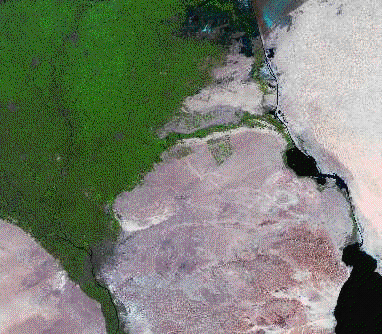
\includegraphics[width=0.88\linewidth]{../images/landsat_mss_september20_1984_nile_delta} \caption{Landsat MSS image acquired September 20, 1984 over the Nile Delta area.}\label{fig:historical-landsat}
\end{figure}

\end{columns}
\end{frame}

\begin{frame}{Meaning}
\protect\hypertarget{meaning}{}
\begin{itemize}
\tightlist
\item
  Remote sensing provides data at a
  synoptic\footnote[frame]{Pertaining to or affording an overall view; referring to the use of meteorological data obtained simultaneously over a wide area for the purpose of presenting a comprehensive and nearly instantaneous picture of the state of the atmosphere}
  global level that is impossible to replicate with in situ
  measurements.
\item
  As developments in novel image processing algorithms and community
  around use and communication of image data continue, scientific value
  of remotely sensed data grow to the extent that never anticipated
  information are extracted.
\item
  However, there are tradeoffs between the local detail of the
  measurements (radiometric resolution, number of spectral bands) and
  the spatial scale of the area being measured.
\item
  Remote sensing is a more rapid means to sample multiple crop
  parameters from spectral indices such as NDVI.

  \begin{itemize}
  \tightlist
  \item
    Productive canopy surface (LAI)
  \item
    Productivity and yield potential
  \item
    Photosynthetic capacity
  \end{itemize}
\end{itemize}
\end{frame}

\begin{frame}{Landsat imagery}
\protect\hypertarget{landsat-imagery}{}
\begin{itemize}
\tightlist
\item
  2022 marks 50th anniversary of the continuous planetary land coverage
  gathered by the Landsat imaging system.
\item
  Instruments on the Landsat satellites have acquired millions of images
  and can be viewed through the U.S. Geological Survey (USGS)
  ``EarthExplorer'' \footnote[frame]{https://earthexplorer.usgs.gov/}
  website.
\item
  Current version of the landsat (Landsat-9) was launched in September
  27, 2021
\item
  Currently Landsat program is managed jointly by:

  \begin{itemize}
  \tightlist
  \item
    NASA
  \item
    USGS
  \end{itemize}
\item
  Landsat 7 data has eight spectral bands with spatial resolutions
  ranging from 15 to 60 m (49 to 197 ft); the temporal resolution is 16
  days.
\item
  Landsat images are usually divided into scenes for easy downloading.
  Each Landsat scene is about 115 miles long and 115 miles wide (or 185
  kilometers long and 185 kilometers wide).
\item
  Landsat imagery is coarse in spatial resolution compared to using
  other remote sensing methods, such as imagery from airplanes.
\end{itemize}
\end{frame}

\begin{frame}{Applications of Landsat imagery}
\protect\hypertarget{applications-of-landsat-imagery}{}
\begin{itemize}
\tightlist
\item
  Agriculture risk management
\item
  Government mapping
\item
  Agricultural water use monitoring
\item
  Global security monitoring
\item
  Support for fire management
\item
  Detection of forest fragmentation
\item
  Detection of forest change
\item
  World agriculture supply and demand estimates
\item
  Vineyard management and water conservation
\item
  Flood mitigation mapping
\item
  Agricultural commodities mapping
\item
  Waterfowl habitat mapping and monitoring
\item
  Coastal change analysis
\item
  Forest health monitoring
\item
  Wildfire risk assessment
\item
  Fisheries, forestry, shrinking inland water bodies, fire damage,
  glacier retreat, urban development, and discovery of new species
\end{itemize}
\end{frame}

\begin{frame}{}
\protect\hypertarget{section}{}
\begin{table}

\caption{\label{tab:unnamed-chunk-1}Landsat 8 Operational Land Imager (OLI) and Thermal Infrared Sensor (TIRS). TIRS bands are acquired at 100 meter resolution, but are resampled to 30 meter in delivered data product}
\centering
\fontsize{8}{10}\selectfont
\begin{tabular}[t]{>{\raggedright\arraybackslash}p{14em}>{\raggedright\arraybackslash}p{10em}>{\raggedright\arraybackslash}p{10em}}
\toprule
Bands & Wavelength (micrometers) & Resolution (meters)\\
\midrule
Band 1 - Ultra Blue (coastal/aerosol) & 0.435 – 0.451 & 30\\
Band 2 - Blue & 0.452 – 0.512 & 30\\
Band 3 - Green & 0.533 – 0.590 & 30\\
Band 4 – Red & 0.636 – 0.673 & 30\\
Band 5 – NIR & 0.851 – 0.879 & 30\\
\addlinespace
Band 6 – SWIR 1 & 1.566 – 1.651 & 30\\
Band 7 – SWIR 2 & 2.107 – 2.294 & 30\\
Band 8 – Panchromatic & 0.503 – 0.676 & 15\\
Band 9 – Cirrus & 1.363 – 1.384 & 30\\
Band 10 – Thermal 1 & 10.60 – 11.19 & 100* (30)\\
\addlinespace
Band 11 – Thermal 2 & 11.50 – 12.51 & 100* (30)\\
\bottomrule
\end{tabular}
\end{table}
\end{frame}

\begin{frame}{}
\protect\hypertarget{section-1}{}
\begin{figure}
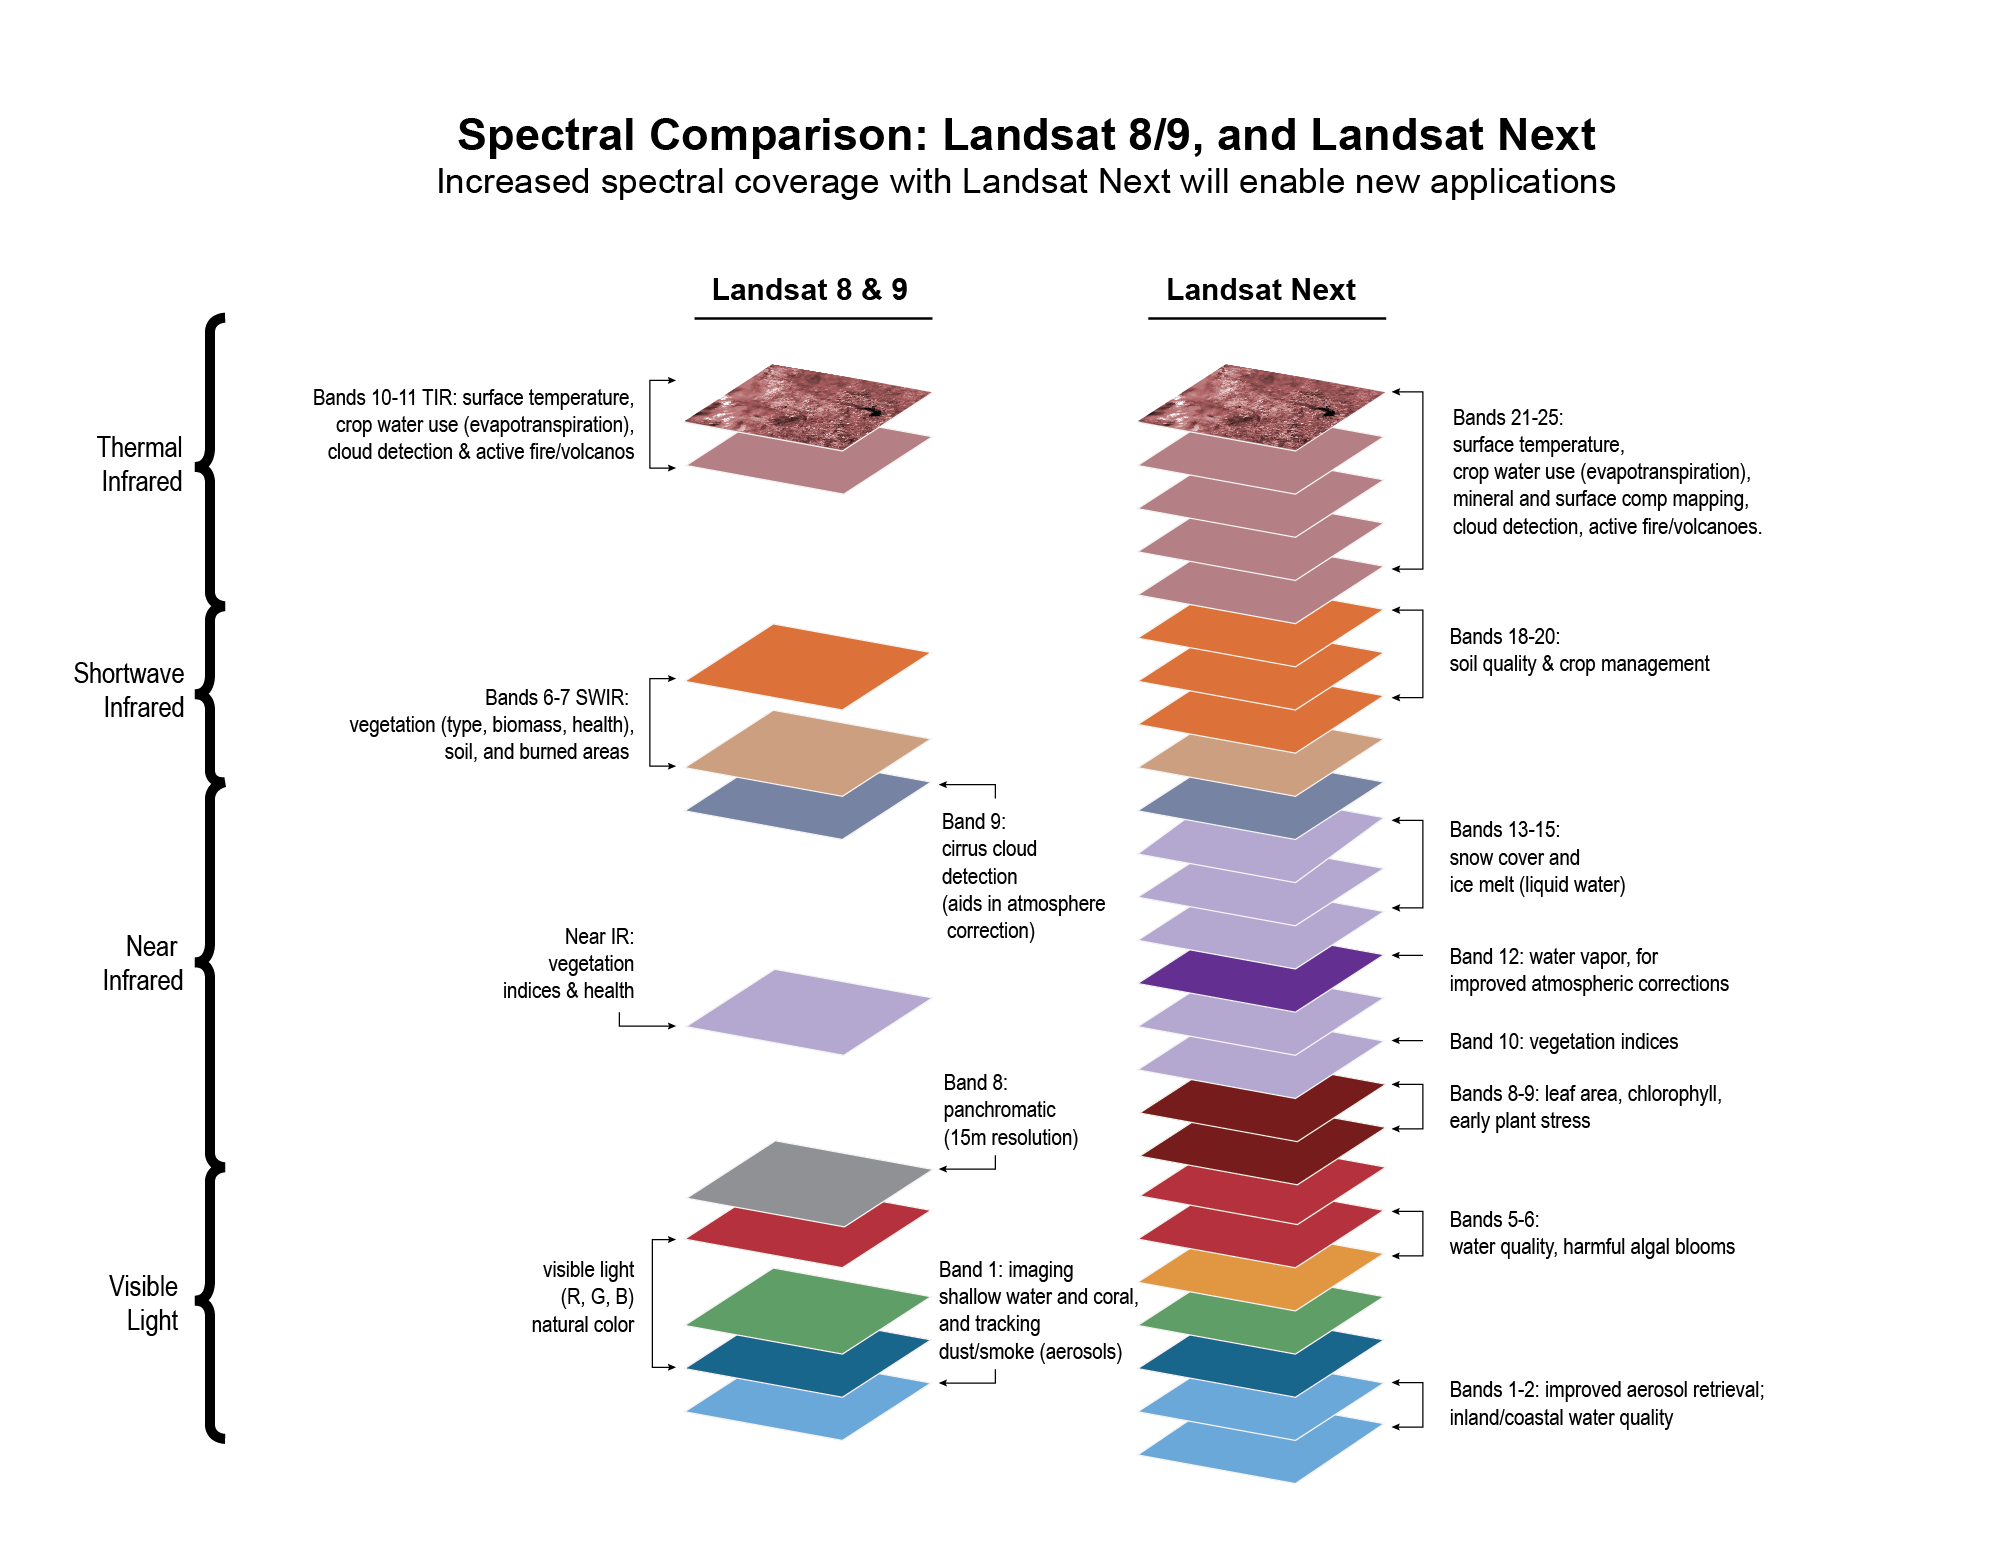
\includegraphics[width=0.65\linewidth]{../images/L8and9-to-LandsatNext-BandComparison} \caption{Source: \url{https://upload.wikimedia.org/wikipedia/commons/8/88/L8and9-to-LandsatNext-BandComparison.png}}\label{fig:band-comparison-lansat89-landsatnext}
\end{figure}
\end{frame}

\hypertarget{acquiring-remotely-sensed-data}{%
\section{Acquiring remotely sensed
data}\label{acquiring-remotely-sensed-data}}

\begin{frame}{Landsat Missions of USGS}
\protect\hypertarget{landsat-missions-of-usgs}{}
\begin{columns}[T, onlytextwidth]

\column{0.5\textwidth}


\begin{center}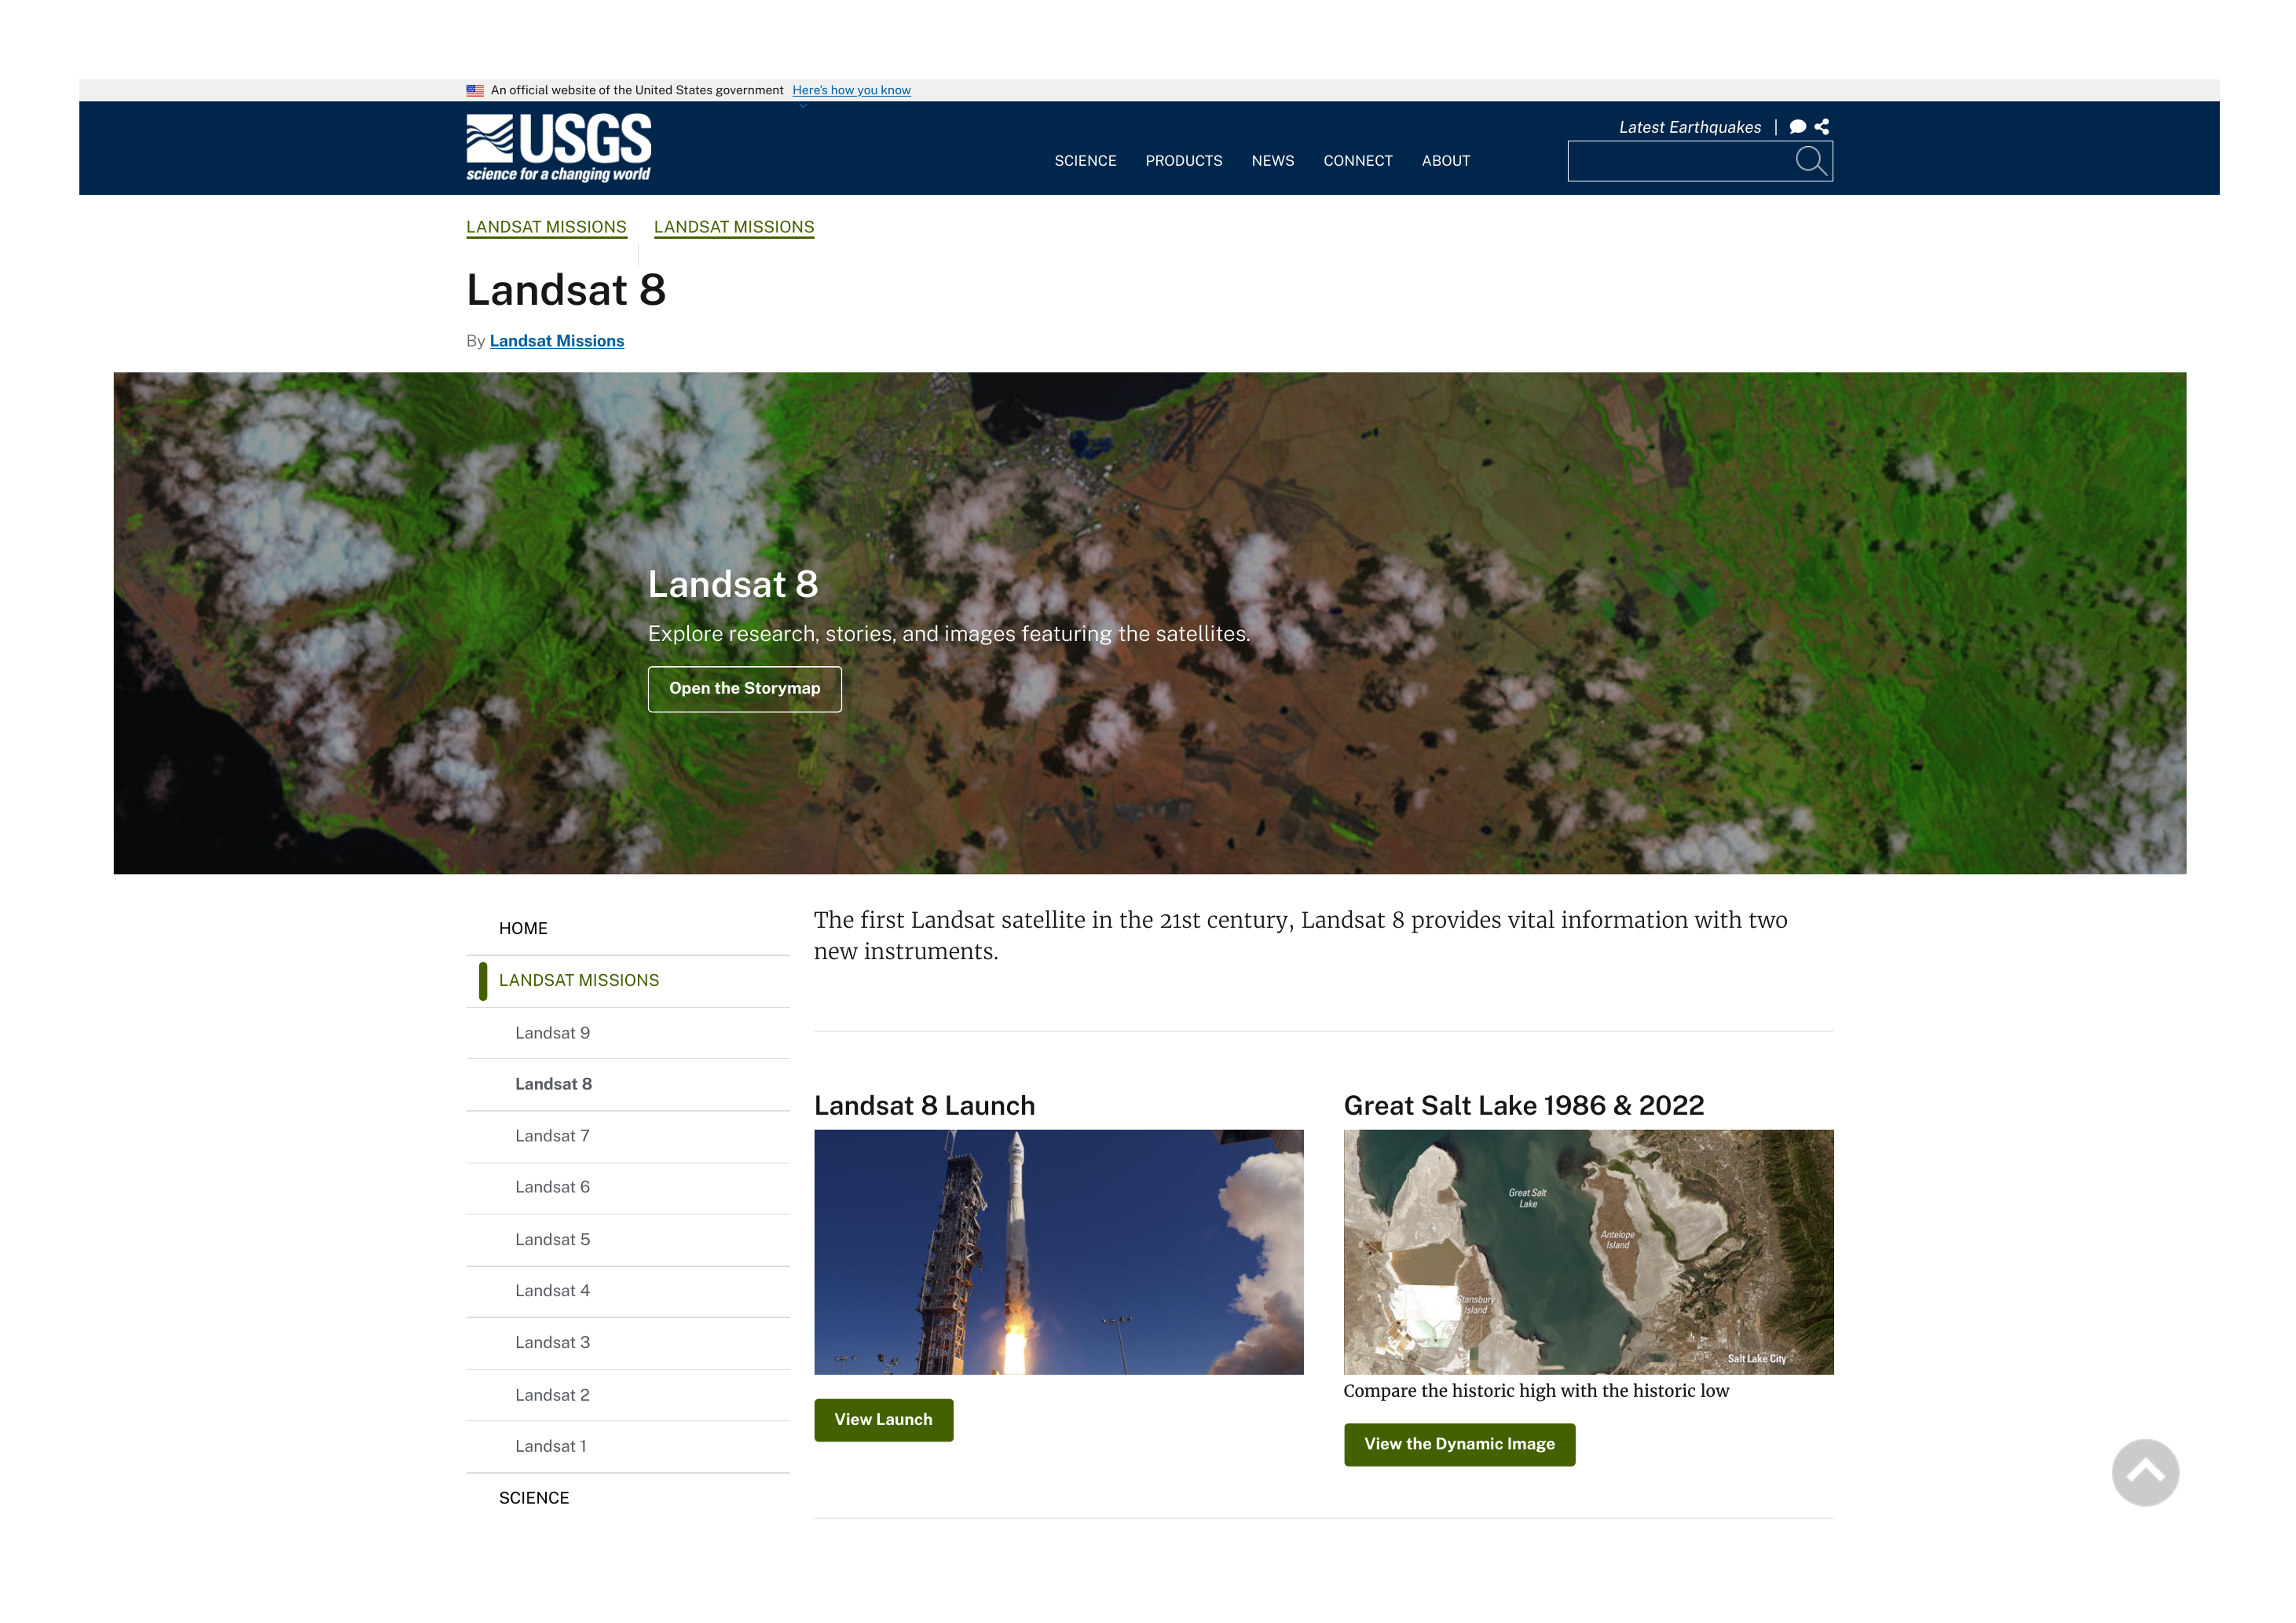
\includegraphics[width=0.98\linewidth]{../images/usgs_official_portal_p1} \end{center}

\column{0.5\textwidth}



\begin{center}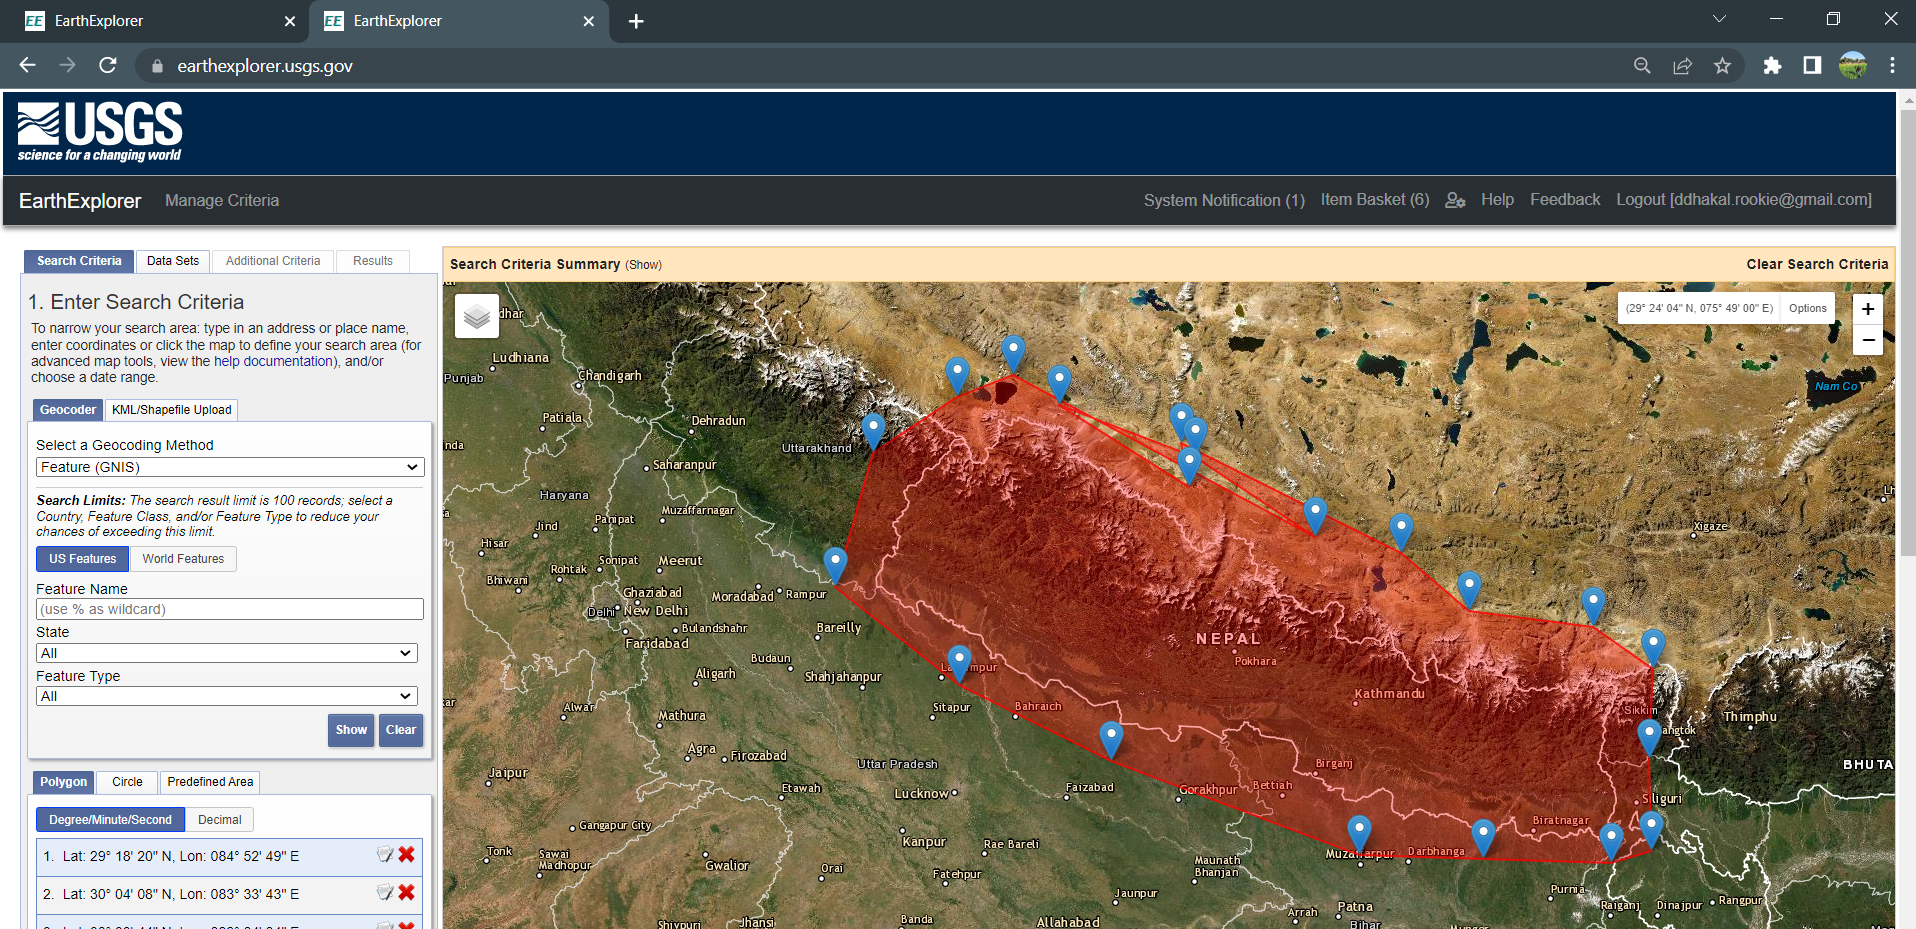
\includegraphics[width=0.98\linewidth]{../images/usgs_landsat_mapping_earth_explorer} \end{center}

\end{columns}
\end{frame}

\begin{frame}{Sentinel mission of NASA}
\protect\hypertarget{sentinel-mission-of-nasa}{}
\begin{center}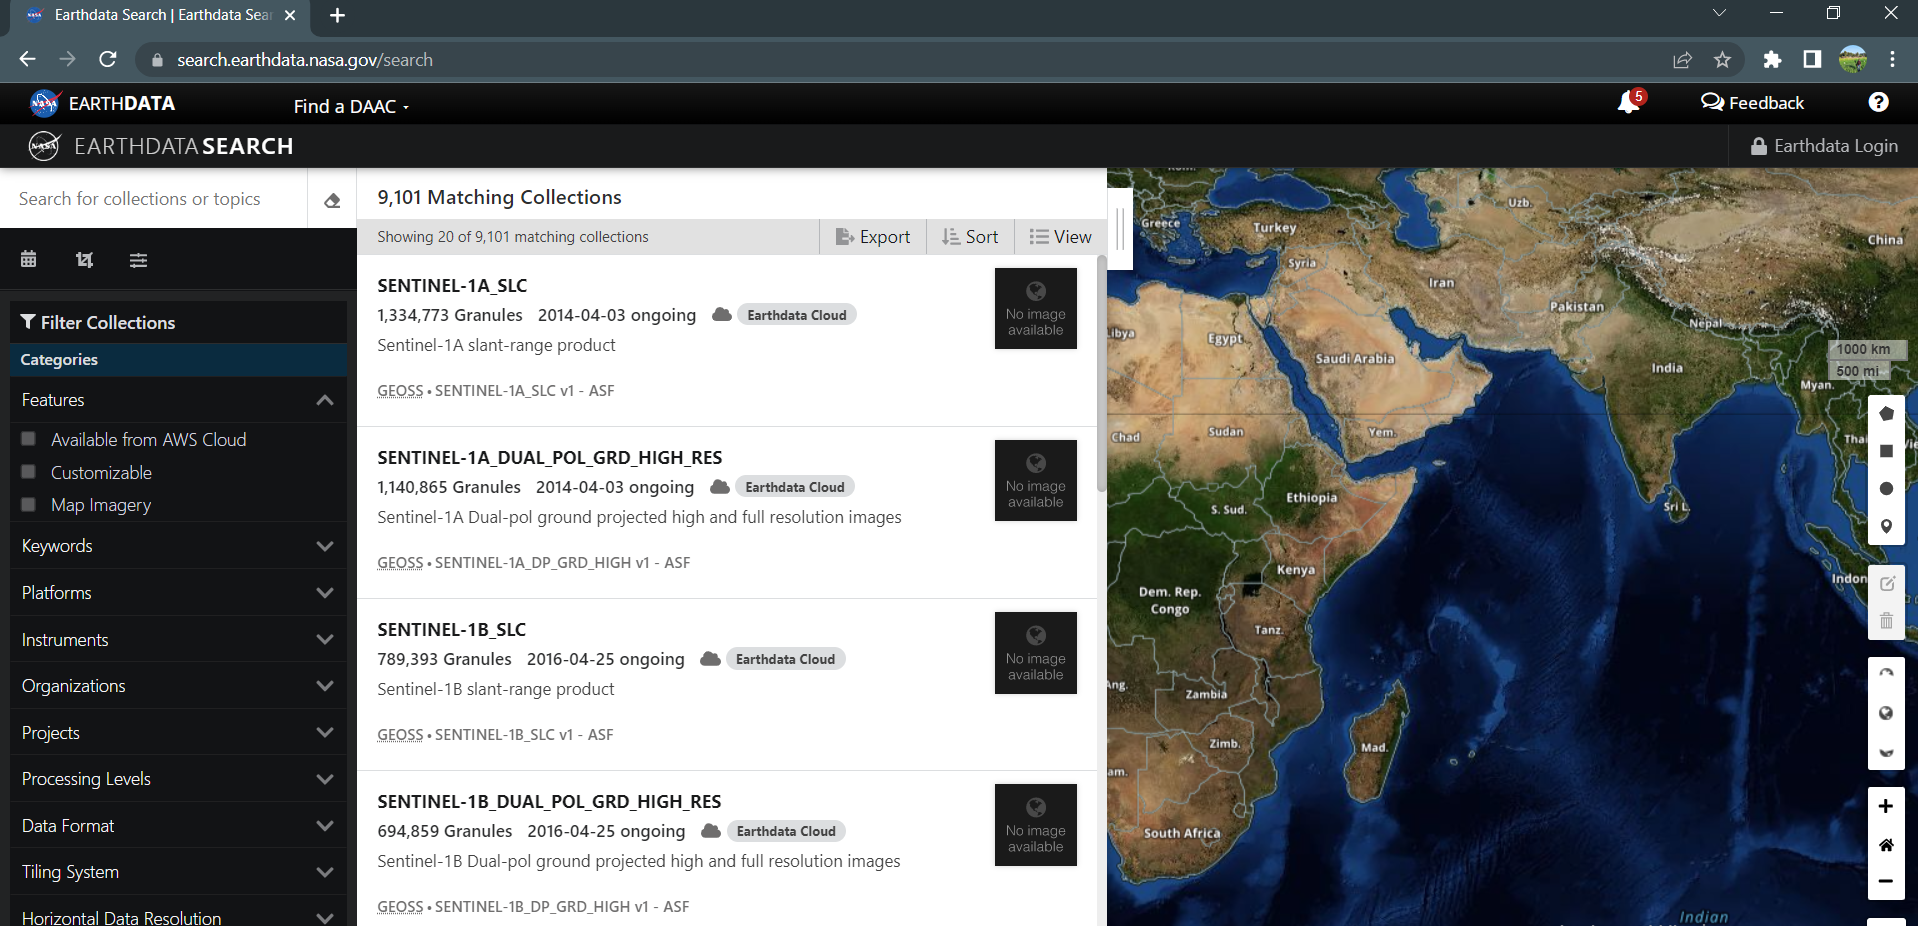
\includegraphics[width=0.85\linewidth]{../images/earthdata_nasa_sentinel_data_viewer} \end{center}
\end{frame}

\hypertarget{image-processing}{%
\section{Image processing}\label{image-processing}}

\begin{frame}{Preprocessing}
\protect\hypertarget{preprocessing}{}
\begin{itemize}
\tightlist
\item
  To remove noise and increase the interpretability of image data
  (essential when a time series of imagery is used or when when multiple
  image operation such as join is required to account for an area
  encompassed by many images to make these images compatible spatially
  and spectrally)
\item
  All images after image preprocessing should appear as if they were
  acquired from the same sensor (Hall et al.~1991).
\item
  Image processing sensors are usually categorized into levels (0, 1A,
  1B, 2A, 2B, 3A, 3B with image quality gradually increased). For
  example, for most sensors, level 3A means that radiometric correction,
  geometric correction and orthorectification have been processed for
  the images.
\item
  Factors such as seasonal phenology, ground conditions and atmospheric
  conditions can contribute to variability in multi-temporal spectral
  responses that may have little to do with the remote sensed objects
  themselves (Song and Woodcock 2003)
\end{itemize}
\end{frame}

\begin{frame}{}
\protect\hypertarget{section-2}{}
\begin{itemize}
\tightlist
\item
  Image preprocessing commonly comprises a series of operations,

  \begin{itemize}
  \tightlist
  \item
    including but not limited to bad lines replacement,
  \item
    radiometric correction,
  \item
    geometric correction,
  \item
    image enhancement and masking (e.g.~for clouds, water, irrelevant
    features) although variations may exist for images acquired by
    different sensors.
  \item
    bad line replacement (fills in missing lines with the line above,
    below or with an average of the two) to determine the overall
    quality of the images (e.g.~missing data lines) through visually
    previewing the images band-by-band
  \item
    cloud imposes a big noise in mapping vegetation cover for
    identifying and thus has to be removed or masked.

    \begin{itemize}
    \tightlist
    \item
      neural network to detect cloud in SPOT VEGETATION images
    \item
      cloud-free space shuttle photograph to detect and remove (mask)
      unwanted cloud covers in Landsat TM scenes
    \end{itemize}
  \end{itemize}
\end{itemize}
\end{frame}

\begin{frame}{Image pre-processing: Radiometric correction}
\protect\hypertarget{image-pre-processing-radiometric-correction}{}
\begin{itemize}
\tightlist
\item
  radiometric correction normally involves the process of correcting
  radiometric errors or distortions of digital images to improve the
  fidelity of the brightness values. radiometric correction methods
  (absolute and relative correction):

  \begin{itemize}
  \tightlist
  \item
    complex mathematical models that describe the main interactions
    involved (certain parameters (i.e.~the atmospheric composition) must
    be known before applying them).
  \item
    methods based on the observations of reference targets (e.g.~water
    or desert land) whose radiometry is known.
  \end{itemize}
\end{itemize}
\end{frame}

\begin{frame}{Image pre-processing: Geometric correction}
\protect\hypertarget{image-pre-processing-geometric-correction}{}
\begin{itemize}
\tightlist
\item
  geometric correction to avoid geometric distortions from a distorted
  image and is achieved by establishing the relationship between the
  image coordinate system and the geographic coordinate system using the
  calibration data of the sensor, the measured data of position and
  altitude and the ground control points
\end{itemize}

\begin{columns}[T, onlytextwidth]
\column{0.5\textwidth}


\begin{center}\includegraphics[width=0.7\linewidth]{08-remote_sensing_image_processing_files/figure-beamer/geometric-fault-example-1} \end{center}

\column{0.5\textwidth}


\begin{center}\includegraphics[width=0.7\linewidth]{08-remote_sensing_image_processing_files/figure-beamer/geometric-fault-example-correct-1} \end{center}

\end{columns}
\end{frame}

\begin{frame}{Image pre-processing: Image enhancement}
\protect\hypertarget{image-pre-processing-image-enhancement}{}
\begin{itemize}
\tightlist
\item
  image enhancement is aimed to emphasize and sharpen particular image
  features (i.e.~particular species of vegetation) for visualization
  purpose

  \begin{itemize}
  \tightlist
  \item
    gray scale conversion,
  \item
    histogram conversion,
  \item
    color composition,
  \item
    color conversion between red-green-blue (RGB), and
  \item
    hue--saturation--intensity transform (HSI), etc.
  \end{itemize}
\end{itemize}
\end{frame}

\hypertarget{bibliography}{%
\section{Bibliography}\label{bibliography}}

\begin{frame}{References}
\protect\hypertarget{references}{}
\end{frame}




\end{document}
